\chapter{Dataset}\label{s:ds}

\section{Introduction}\label{s:ds-intro}

As I explained in the Abstract, I chose \modanet after having looked at many others.

An interesting one I found, for example, was DeepFashion \cite{DeepFashion2}, but it didn't feature any footwear annotations unfortunately -- which were the main focus of the task I was given. It had over 800 thousand images though!

\begin{figure}[H]
	\centering
	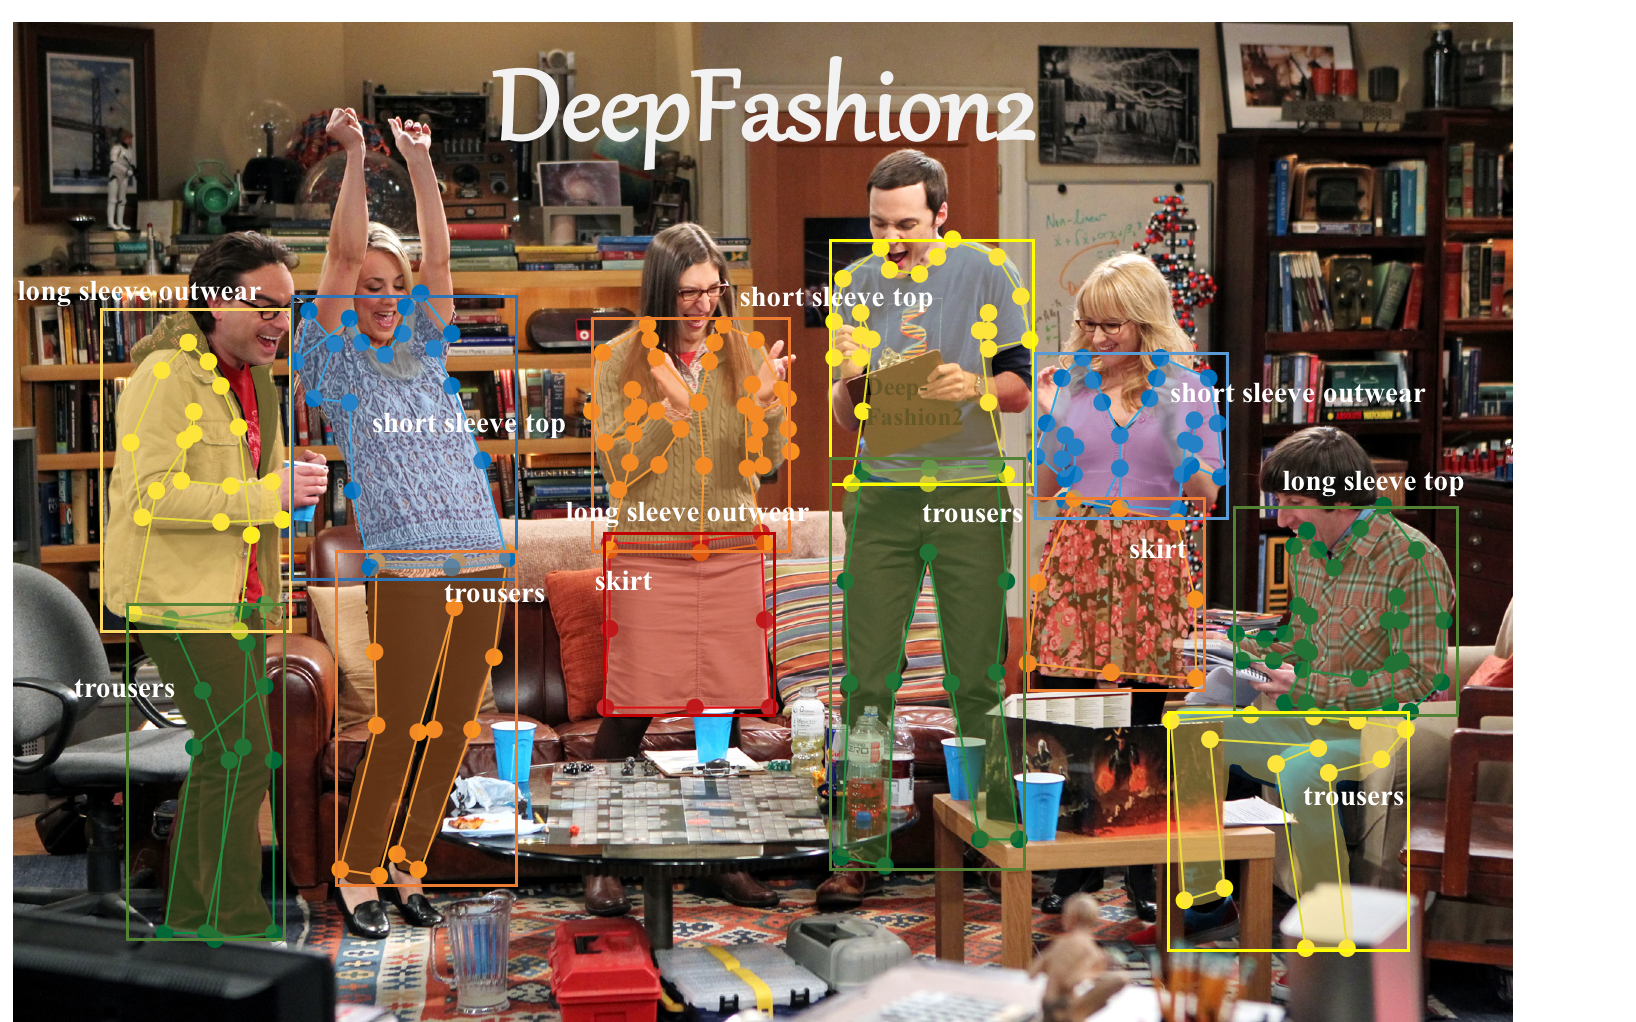
\includegraphics[width=0.75\textwidth]{images/deepfashion2_bigbang}
	\caption{DeepFashion2 feature image.}
	\label{f:deepfashion2_bigbang}
\end{figure}

But what is a dataset? Simply speaking, a dataset is a collection of data that is usually useful for statistics / data analysis purposes. Many datasets today cannot be fully exploited due to our technology, but this is rapidly changing as we continue to develop new algorithms capable to \emph{generalize} better the features that these datasets expose.

For our task, what we needed was a dataset of real-world images that could ideally differenciate between any model, brand and size of any kind of apparel. That means anything you can wear (and buy) could be retrieved by this ideal model, along with the prices when it was bought and the prices now\dots

Unfortunately, one can dream as big as he wants, but the reality is that \modanet is the best I could find, as you can clearly see below in this comparison between competing datasets.

\begin{table}[H]
	\centering
	\caption{Comparison of ModaNet with other datasets for fashion parsing. ModaNet surpasses previous datasets in terms of annotation granularity and scale. \checkmark$^*$  indicates the annotations are not included in the original dataset. The count of categories excludes non-fashion categories, such as \emph{hair}, \emph{skin}, \emph{face}, \emph{background} and \emph{null}.}
	\label{t:datasets}
	\resizebox{\columnwidth}{!}{
	\begin{tabular}{@{}lcccccc@{}}
		\hline
		& DeepFashion~\cite{liu2016deepfashion} & CFPD~\cite{liu2013fashion}    & CCP~\cite{yang2014clothing}     & Fashionista~\cite{yamaguchi2012parsing} & HPW\cite{liang2015deep} & ModaNet~\cite{Zheng_2018}  \\
		\hline
		\# of images      & $800,000$   & $2,682$ & $1,004$ & $685$       & $1,833$ & $55,176$ \\
		\# of categories  &     50        &     19    &      56   &       53      &  11  & 13  \\
		Pixel annotation & \texttimes      & \checkmark    &\checkmark & \checkmark      &\checkmark & \checkmark      \\
		Bounding box      & landmarks   &  \checkmark$^*$       & \checkmark$^*$         &     \checkmark$^*$         & \checkmark$^*$  & \checkmark      \\
		Polygon           & \texttimes        & \texttimes     & \texttimes     & \texttimes        &\texttimes  & \checkmark      \\ 
		\hline
	\end{tabular}
	}
\end{table}

Then I stumbled upon this great dataset. It had much richer annotations, with \emph{almost-perfect} and very precise masks for each instance, plus it included footwear too!
\modanet has been annotated and managed by eBay researchers.
Here is their brief description of their work (on their GitHub page):
\begin{quotation}
	ModaNet is a street fashion images dataset consisting of annotations related to RGB images. ModaNet provides multiple polygon annotations for each image. This dataset is described in a technical paper with the title \emph{ModaNet: A Large-Scale Street Fashion Dataset with Polygon Annotations} \cite{zheng/2018acmmm}. Each polygon is associated with a label from 13 meta fashion categories. The annotations are based on images in the PaperDoll image set, which has only a few hundred images annotated by the superpixel-based tool. The contribution of ModaNet is to provide new and extra polygon annotations for the images.
\end{quotation}


\section{PaperDoll}\label{s:ds-paperdoll}

The PaperDoll dataset \cite{yamaguchi2013paper} is an expansion of the Fashionista dataset \cite{yamaguchi2012parsing}, which were all developed without deep learning in mind. In fact, they initially used HOGs, cited briefly in \sref{s:nnevo-intro}. They only managed to do \emph{Semantic Segmentation} [\sref{s:patt-sema}] though.

\begin{figure}[H]
	\centering
	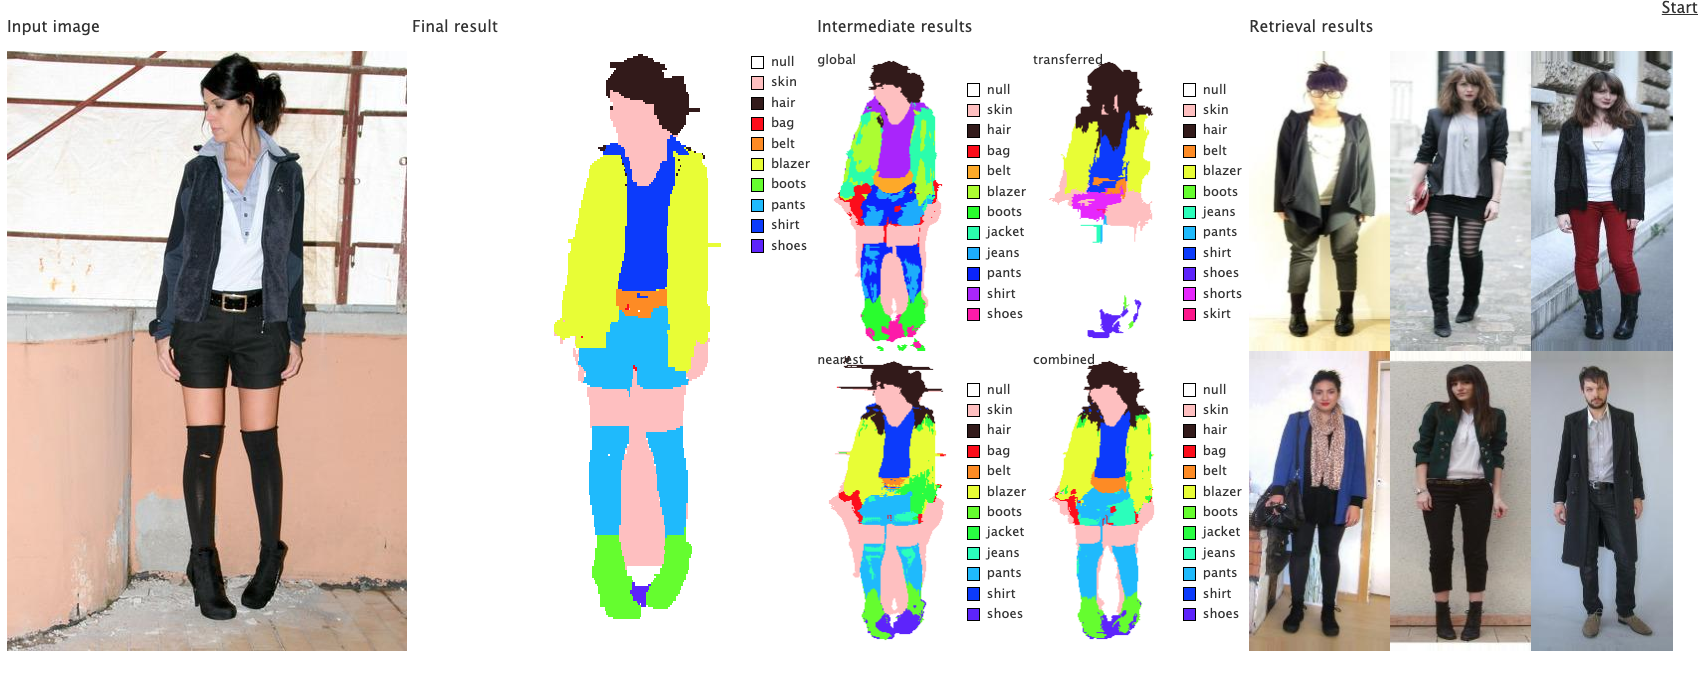
\includegraphics[width=\linewidth]{images/paperdollparsing}
	\caption{Results of the PaperDoll parsing from 2013, still online at \texttt{clothingparsing.com}}
	\label{f:paperdollparsing}
\end{figure}

An interesting thing the PaperDoll dataset added was retrieving related images. In their paper, they acknowledge that many people living in the same environment (i.e. college) also dress in a similar style.

They achieved this with a method that gave the name to the dataset: 
“like laying paper cutouts of clothing items onto a paper doll", each query generates related images that are subsequently fed back to the query to enlarge the database annotation.

\begin{figure}[H]
	\centering
	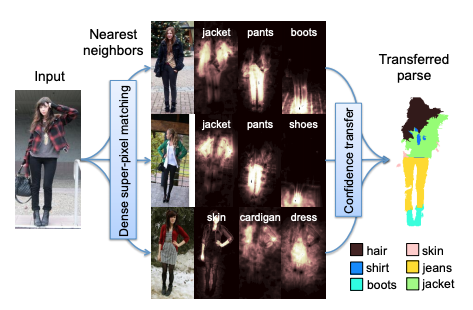
\includegraphics[width=.75\linewidth]{images/paperdolltransfer}
	\caption{Transferred parse. Likelihoods in nearest neighbors are transferred to the input via dense matching.}
	\label{f:paperdolltransfer}
\end{figure}

\subsection{The source: Chictopia}\label{s:ds-paperdoll-chictopia}

\texttt{chictopia.com} is a social network focused on fashion.
The data from the site was not available until January \nth{31}, 2019. It was crawled originally in Fall 2012.
That is the date when, thanks to the new copyright law in Japan \footnote{European Alliance for Research Exellence, September \nth{3}, 2018: \emph{Japan amends its copyright legislation to meet future demands in AI and big data}}  , the researchers decided to release the raw dataset for research purposes.

Thanks to this we can enjoy training our algorithms on the raw paperdoll data annotated with \modanet.

\subsection{The RAW Data}\label{s:ds-paperdoll-raw}

The raw data is available on the paperdoll GitHub repo, along with the instructions to download the images.
The dataset requires SQLite3 and LMDB. After you download the ~40GB database file, you have to extract it and then the images are encapsulated in the database with some labels (not anywhere rich as the ModaNet ones, nor in the COCO format ready to be trained).
For example, you could retrieve all the photos taken by a particulare chictopia user (not very useful). Or you could use the post tag relationships, which I have not used—but they could become very useful for future work!

Here are the post tag relationships, retrievable in SQL style:
\begin{itemize}
	\item Color: color of the item.
	\item Style: general style of the post.
	\item Occasion: occasion of the outfit.
	\item Clothing: type of the item.
	\item Brand: brand of the item.
	\item Trend: free-form tag.
\end{itemize}

I think in particular, \emph{Brand} is definitely the most interesting one, especially because of the original intent of this thesis, explained in the Introduction. The \emph{Occasion} could also be useful in determining where an item is worn.

% TODO explain in intro Adidas focus

There are also relationships between users. A user has many friends and fans, so in theory you could track how well a \emph{Creator}, which in italy are called \emph{Influencers}, has been “selling" the items he or she is sponsoring!

All it's needed is to integrate the \modanet annotations with the sparse information on the paperdoll SQL database and add a dataset comprising of the specific models of each clothing and apparel item. (this sounds too simple I know)

% TODO link to conclusions

\section{ModaNet}\label{s:ds-modanet}

\begin{quotation}
	“Clothing recognition is a challenging and societally important problem – global sales for clothing total over a hundred billion dollars, much of which is conducted online." \cite{yamaguchi2013paper}
\end{quotation}

\begin{table}[H]
\centering
\small
\caption{\textbf{ModaNet labels}. Meta categories are groups of highly related raw categories}
\label{t:modanet statistics}
\begin{tabularx}{\textwidth}{@{}lXccc@{}}
\hline
Meta & Raw & \#Train & \#Val & Avg Inst. size\\
\hline
bag  & bag & $36,699$  & $2,155$  & 4.88\% \\
belt  & belt & $13,743$ & $771$ & 0.46\% \\
boots  & boots & $7,068$ & $691$ & 2.40\%  \\
footwear  & footwear & $39,364$ & $1,617$ & 0.96\% \\
outer  & coat, jacket, suit, blazers
%, cardigan, sweater, jumpsuits, rompers, vest 
& $23,743$ & $1,358$ & 7.48\% \\
dress  & dress, t-shirt dress & $14,460$ & $804$ & 10.49\% \\
sunglasses  & sunglasses &  $8,780$ & $524$ & 0.31\% \\
pants  & pants, jeans, leggings & $23,075$  &  $1,172$ & 5.65\% \\
top  & top, blouse, t-shirt, shirt & $34,745$ & $1,862$ & 4.83\% \\ 
shorts  & shorts & $5,775$ & $429$ & 2.86\% \\ 
skirt  & skirt & $10,860$  & $555$ &  6.40\% \\ 
headwear  & headwear & $5,405$ & $491$ & 1.25\% \\ 
scarf\&tie  & scarf, tie & $3,990$ & $378$ & 2.55\%  \\ 
\hline
\end{tabularx}
\end{table}

As said above at the end of \sref{s:ds-intro}, \modanet provides high quality annotations to $\sim$50k images on the PaperDoll dataset. The annotations include masks, bounding boxes and category (label). The labels are defined above in \tref{t:modanet statistics}.

\section{Organizing the Dataset}\label{s:ds-organizing}

\section{A Python Package to automate the process}\label{s:ds-package}